\question 某计算机处理器主频为50MHz,采用定时查询方式控制设备A的I/O,查询程序运行一次所用的时钟周期至少为500。在设备A工作期间,为保证数据不丢失,每秒需对其查询至少200次,则CPU用于设备A的I/O的时间占整个CPU时间的百分比至少是(
)
\par\twoch{0.02\%}{0.05\%}{\textcolor{red}{0.20\%}}{0.50\%}
\begin{solution}由于CPU每秒需对其查询至少200次,每次500个时钟周期。所以,CPU用于设备A的I/O时间每秒最少为500×200=100000个时钟周期。故CPU用于设备A的I/O的时间占整个CPU时间的百分比至少为
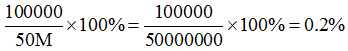
\includegraphics[width=3.62500in,height=0.53125in]{computerassets/0b4664d4ddd6eea90c29ef97b411070e.jpeg}
【总结】
程序查询方式:数据在CPU和外部设备之间的传送完全靠计算机程序控制,其核心思想是每时每刻CPU需要不断查询I/O设备是否准备就绪。如果没有准备就绪,就不断等待,只有设备已做好准备,CPU才能执行I/O指令进行数据传送。
程序查询方式存在着以下明显的缺点。
1)在查询过程中,CPU长期处于``踏步''等待状态,使系统效率大大降低。
2)CPU在一段时间内只能和一台外设交换信息,其他设备不能同时工作。
\end{solution}
